\documentclass[11pt, a4paper]{article}

%% ── Packages ─────────────────────────────────────────────────────────────────
\usepackage[a4paper, top=2.5cm, bottom=2.5cm, left=2.8cm, right=2.8cm, headheight=14pt]{geometry}
\usepackage[T1]{fontenc}
\usepackage[utf8]{inputenc}
\usepackage{lmodern}
\usepackage{microtype}
\usepackage{setspace}
\usepackage{parskip}
\usepackage{titlesec}
\usepackage{booktabs}
\usepackage{array}
\usepackage{graphicx}
\usepackage{float}
\usepackage{caption}
\usepackage{amsmath}
\usepackage{amssymb}
\usepackage{bm}
\usepackage{xcolor}
\usepackage{hyperref}
\usepackage{fancyhdr}
\usepackage{enumitem}
\usepackage{tcolorbox}
\usepackage{colortbl}
\usepackage{eurosym}
\usepackage{natbib}

%% ── Colours ──────────────────────────────────────────────────────────────────
\definecolor{navyblue}{RGB}{31,58,95}
\definecolor{burntorange}{RGB}{224,123,57}
\definecolor{forestgreen}{RGB}{46,139,87}
\definecolor{darkred}{RGB}{139,26,26}
\definecolor{midgrey}{RGB}{110,110,110}

\hypersetup{colorlinks=true,linkcolor=navyblue,citecolor=navyblue,
  urlcolor=burntorange,pdftitle={VWCE.DE DCA Investment Forecast}}

%% ── Typography ───────────────────────────────────────────────────────────────
\setstretch{1.18}
\titleformat{\section}{\large\bfseries\color{navyblue}}{\thesection.}{0.65em}{}
  [\vspace{-0.4em}\color{navyblue}\rule{\linewidth}{0.9pt}\vspace{0.15em}]
\titleformat{\subsection}{\normalsize\bfseries\color{navyblue}}{\thesubsection.}{0.55em}{}
\titleformat{\subsubsection}{\normalsize\itshape\color{navyblue}}{\thesubsubsection.}{0.5em}{}
\titlespacing{\section}{0pt}{1.6em}{0.5em}
\titlespacing{\subsection}{0pt}{1.1em}{0.3em}

%% ── Header / footer ──────────────────────────────────────────────────────────
\pagestyle{fancy}\fancyhf{}
\lhead{\small\color{navyblue}\textbf{VWCE.DE --- DCA Investment Forecast}}
\rhead{\small\color{navyblue}Quantitative Analysis $\cdot$ June 2026}
\cfoot{\small\color{midgrey}\thepage}
\renewcommand{\headrulewidth}{0.4pt}
\renewcommand{\headrule}{\color{navyblue}\hrule width\headwidth height\headrulewidth}

%% ── Captions ─────────────────────────────────────────────────────────────────
\captionsetup{font=small,labelfont={bf,color=navyblue},labelsep=period,margin=0.4cm,skip=4pt}

%% ── Table helpers ────────────────────────────────────────────────────────────
\newcolumntype{L}[1]{>{\raggedright\arraybackslash}p{#1}}
\newcolumntype{R}[1]{>{\raggedleft\arraybackslash}p{#1}}
\newcommand{\rownavy}{\rowcolor{navyblue!10}}
\newcommand{\rowbest}{\rowcolor{forestgreen!15}}

%% ── Boxes ────────────────────────────────────────────────────────────────────
\tcbuselibrary{skins,breakable}
\newtcolorbox{summarybox}[1][]{enhanced,colback=navyblue!5,colframe=navyblue,
  boxrule=0.7pt,arc=3pt,left=9pt,right=9pt,top=7pt,bottom=7pt,
  fonttitle=\bfseries\color{navyblue},#1}
\newtcolorbox{warnbox}[1][]{enhanced,colback=darkred!4,colframe=darkred,
  boxrule=0.7pt,arc=3pt,left=9pt,right=9pt,top=7pt,bottom=7pt,
  fonttitle=\bfseries\color{darkred},#1}

%% ═════════════════════════════════════════════════════════════════════════════
\begin{document}

%%─── Title page ───────────────────────────────────────────────────────────────
\begin{titlepage}
  \centering\vspace*{1.2cm}
  {\color{navyblue}\rule{\linewidth}{2.5pt}}\vspace{0.7cm}

  {\fontsize{26}{32}\selectfont\bfseries\color{navyblue}
    VWCE.DE Investment Forecast\\[0.45em]}
  {\Large\color{navyblue}
    Econometric Analysis of a Monthly \euro{}1{,}000 DCA Programme\\[0.3em]}
  {\large\color{burntorange}
    Interactive Brokers $\cdot$ \euro{}3 fee/trade $\cdot$
    VWCE TER 0.22\% p.a.\ $\cdot$ Start: September 2027}

  \vspace{0.6cm}{\color{navyblue}\rule{\linewidth}{2.5pt}}\vspace{1.0cm}

  {\small\bfseries\color{navyblue}Results Summary (10{,}000 Monte Carlo paths)}\\[0.5em]
  \begin{tabular}{@{}lR{2.6cm}R{2.6cm}R{2.2cm}R{2.2cm}R{2cm}@{}}
    \toprule
    \textbf{Horizon} & \textbf{Capital} & \textbf{Median Portfolio} & \textbf{P(loss)} & \textbf{XIRR} & \textbf{Multiple}\\
    \midrule
    1 year   & \euro{}12{,}000  & \euro{}12{,}699      & 27.7\% & 12.32\% & 1.06$\times$\\
    3 years  & \euro{}36{,}000  & \euro{}42{,}104      & 18.7\% & 11.28\% & 1.17$\times$\\
    5 years  & \euro{}60{,}000  & \euro{}77{,}663      & 14.0\% & 10.95\% & 1.29$\times$\\
    10 years & \euro{}120{,}000 & \euro{}200{,}133     &  7.9\% & 10.30\% & 1.67$\times$\\
    20 years & \euro{}240{,}000 & \euro{}696{,}587     &  3.5\% &  9.76\% & 2.90$\times$\\
    30 years & \euro{}360{,}000 & \euro{}1{,}913{,}813 &  2.0\% &  9.51\% & 5.32$\times$\\
    \bottomrule
  \end{tabular}

  \vfill{\small\color{midgrey}
    Prepared: 18 June 2026 \quad\textbar\quad
    Data: VWCE.DE + VT (Jun 2008--Jun 2026, 4{,}540 obs) \quad\textbar\quad
    GJR-GARCH(1,2)-$t$ + Merton jump-diffusion + Bayesian drift
  }
\end{titlepage}

\tableofcontents\newpage

%%─── Section 1 ────────────────────────────────────────────────────────────────
\section{Asset and Data}

\subsection{VWCE.DE}

Vanguard FTSE All-World UCITS ETF (VWCE.DE, Xetra) is an EUR-denominated accumulating ETF tracking the FTSE All-World Index ($\approx$3{,}700 equities across 49 markets). AUM: $\approx$\euro{}66 billion. TER: 0.22\% p.a., continuously deducted from NAV and modelled as a daily drag of $0.22\%/252$ in all simulations. Latest price: \euro{}165.46 (18 June 2026), +202.7\% since inception at \euro{}54.66 in July 2019.

\subsection{Extended Calibration Sample (2008--2026)}

VWCE has traded since July 2019. Seven years of data excludes the GFC and several other major corrections that are essential for calibrating long-run volatility. We splice in Vanguard VT (ARCA, USD), which tracks the same FTSE All-World Index since June 2008, converting to EUR at daily EUR/USD spot rates and rescaling by 1.203 at the splice point. The resulting sample spans June 2008 to June 2026 (4{,}540 observations).

\begin{figure}[H]\centering
  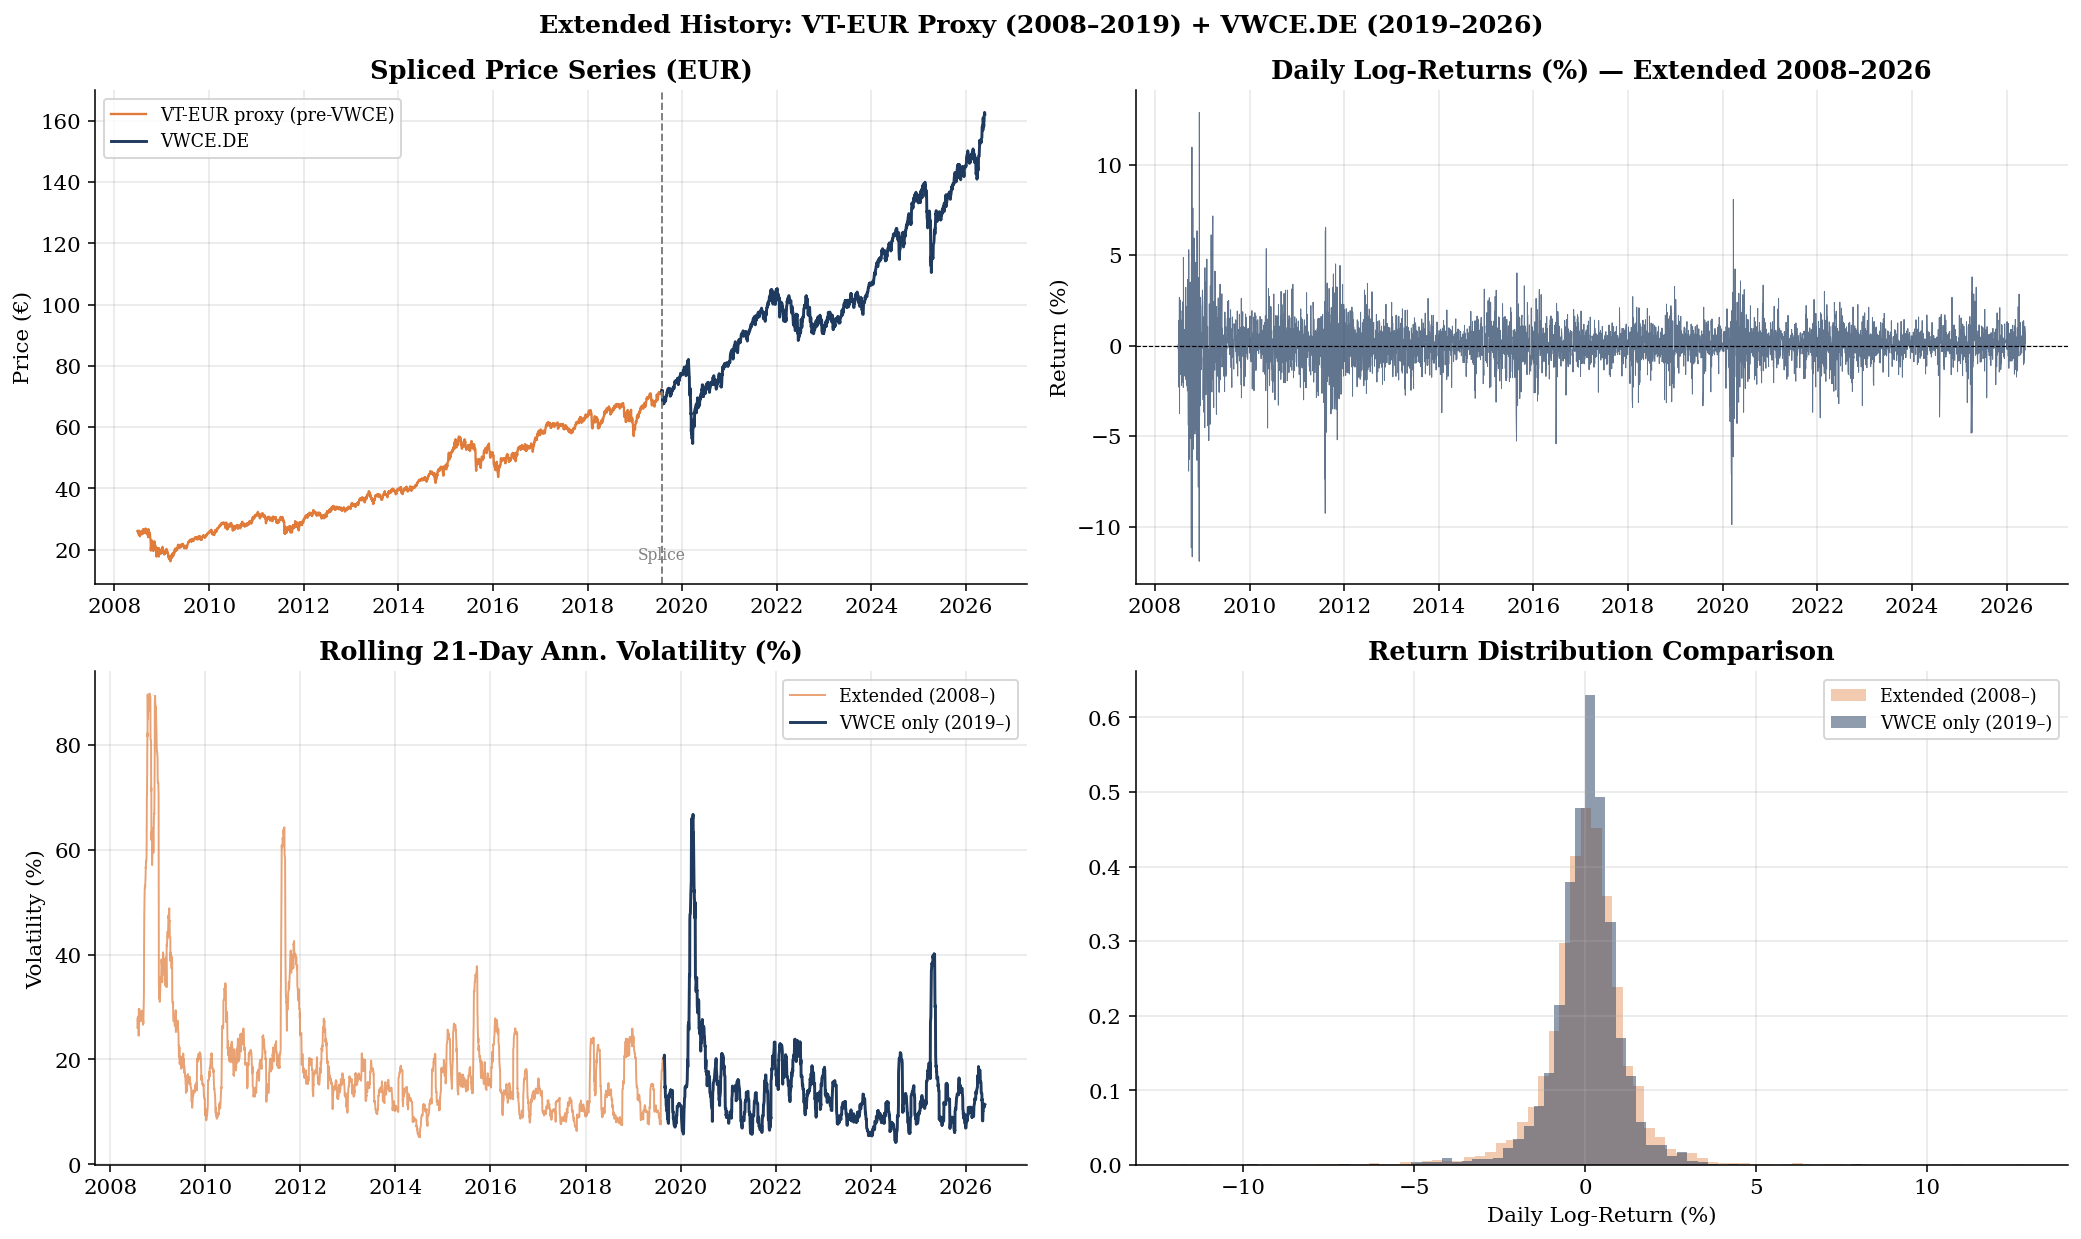
\includegraphics[width=\linewidth]{v2_fig1_extended_history.png}
  \caption{VT-EUR proxy (2008--2019, orange) spliced with VWCE.DE (2019--2026, blue). The GFC drives rolling volatility above 80\% annualised, far beyond anything in the 7-year VWCE window. The extended return distribution has heavier tails and a wider body.}
  \label{fig:ext}
\end{figure}

\begin{table}[H]\centering
  \caption{Descriptive Statistics: Extended vs VWCE-only Sample}\label{tab:stats}
  \begin{tabular}{@{}L{5.5cm}R{3cm}R{3cm}@{}}
    \toprule\textbf{Statistic}&\textbf{Extended (2008--2026)}&\textbf{VWCE only (2019--2026)}\\\midrule
    Observations           & 4{,}539  & 1{,}750\\
    Annualised return      & 10.28\%  & 11.84\%\\
    Annualised volatility  & 20.35\%  & 16.29\%\\
    Sharpe ratio           & 0.505    & 0.727\\
    Skewness               & $-$0.580 & $-$1.062\\
    Excess kurtosis        & 12.955   & 11.525\\
    \bottomrule
  \end{tabular}
\end{table}

\subsection{Exploratory Analysis}

\begin{figure}[H]\centering
  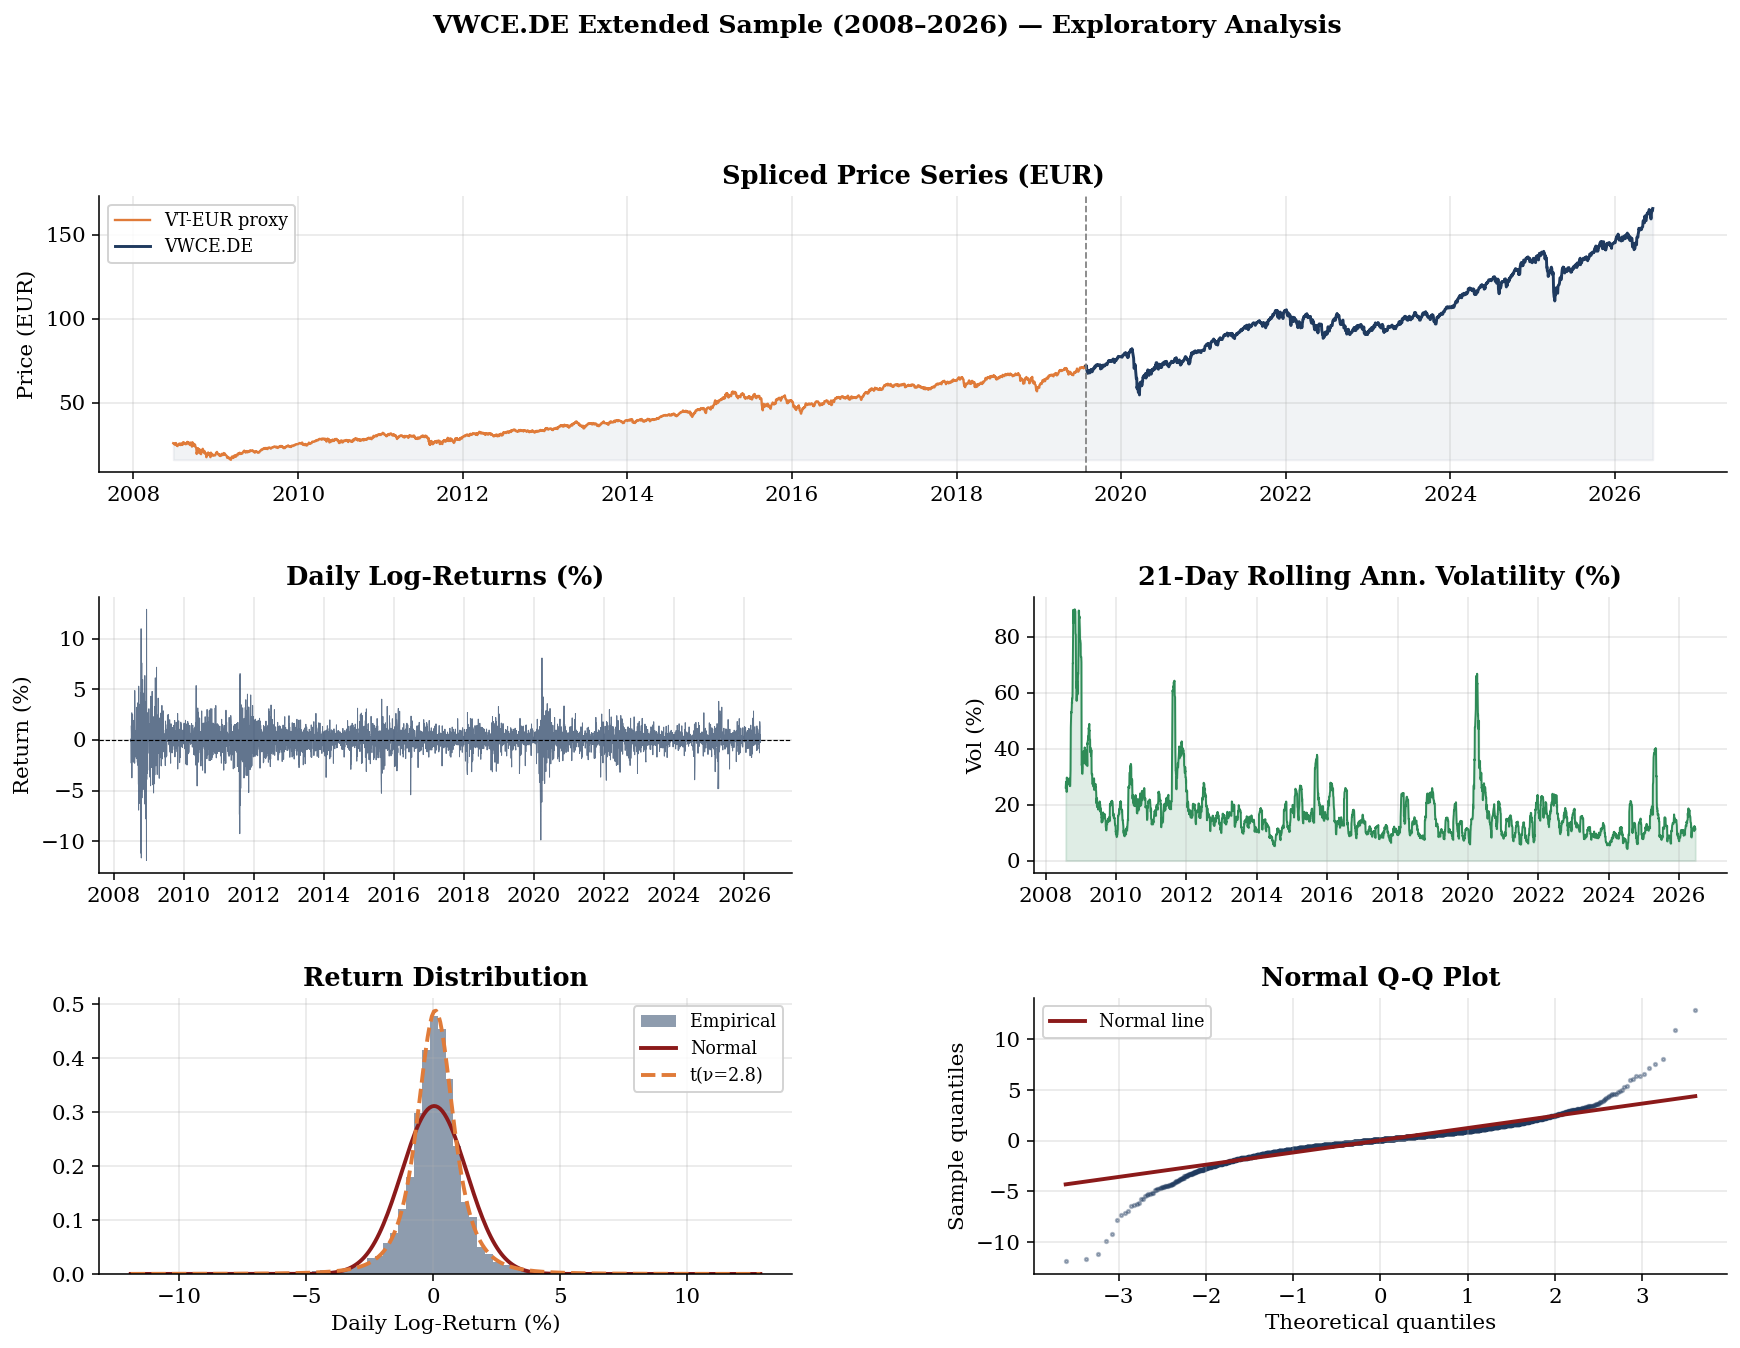
\includegraphics[width=\linewidth]{fig1_eda.png}
  \caption{Exploratory analysis of the extended sample. \textit{Top}: spliced price series (orange = VT-EUR; blue = VWCE.DE). \textit{Middle}: daily log-returns and rolling 21-day annualised volatility. \textit{Bottom left}: empirical distribution vs Normal and Student-$t$ fits --- fat tails are clearly visible. \textit{Bottom right}: Normal Q-Q plot confirms extreme leptokurtosis.}
  \label{fig:eda}
\end{figure}

\begin{figure}[H]\centering
  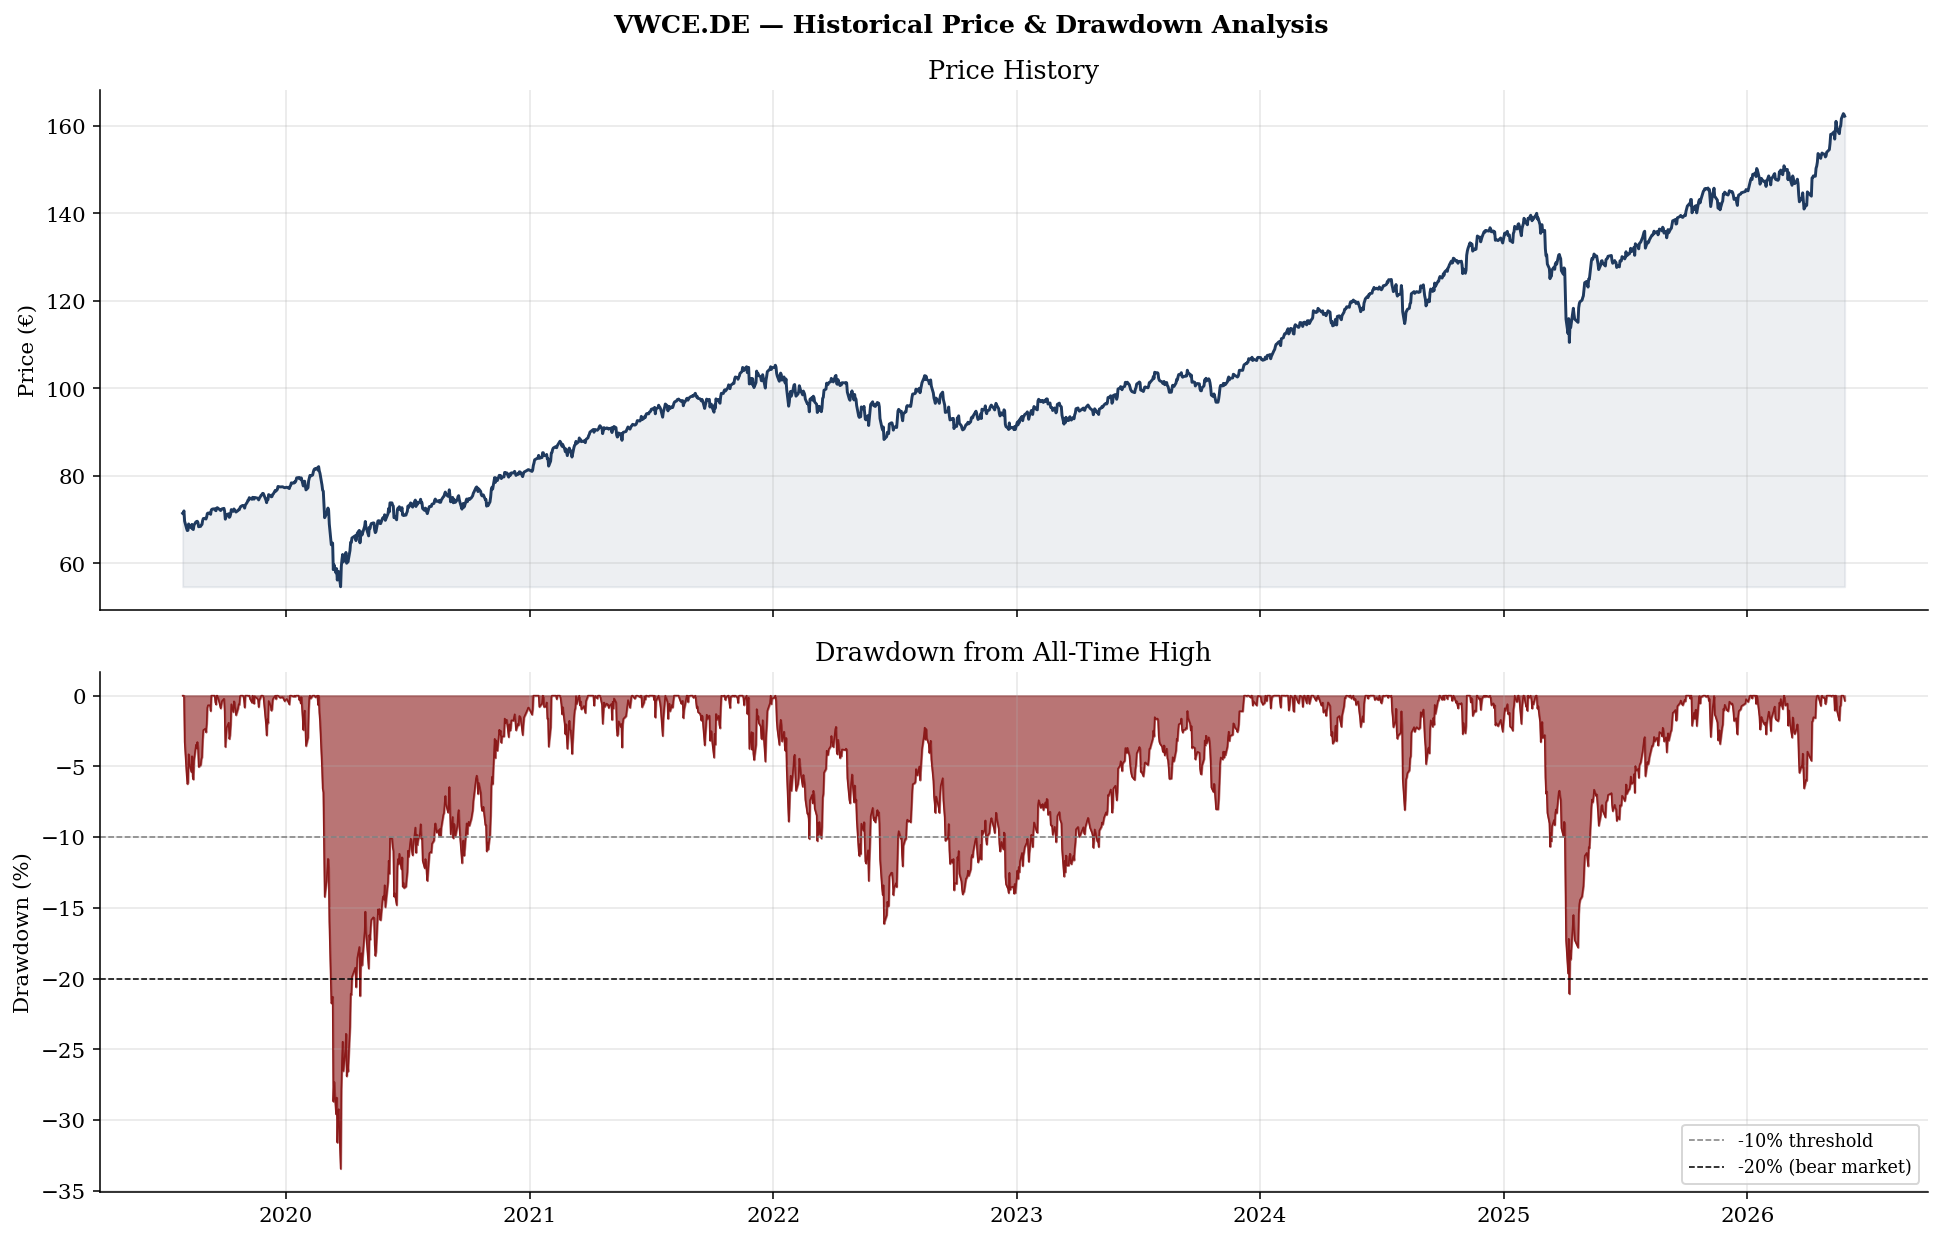
\includegraphics[width=\linewidth]{fig7_drawdown.png}
  \caption{VWCE.DE price history and drawdown from all-time high. Three drawdown episodes: COVID ($-$33.4\%), 2022 rate-shock ($\approx -$20\%), 2025 turbulence ($\approx -$15\%). All recovered. Current drawdown: $-$0.4\%.}
  \label{fig:drawdown}
\end{figure}

\begin{figure}[H]\centering
  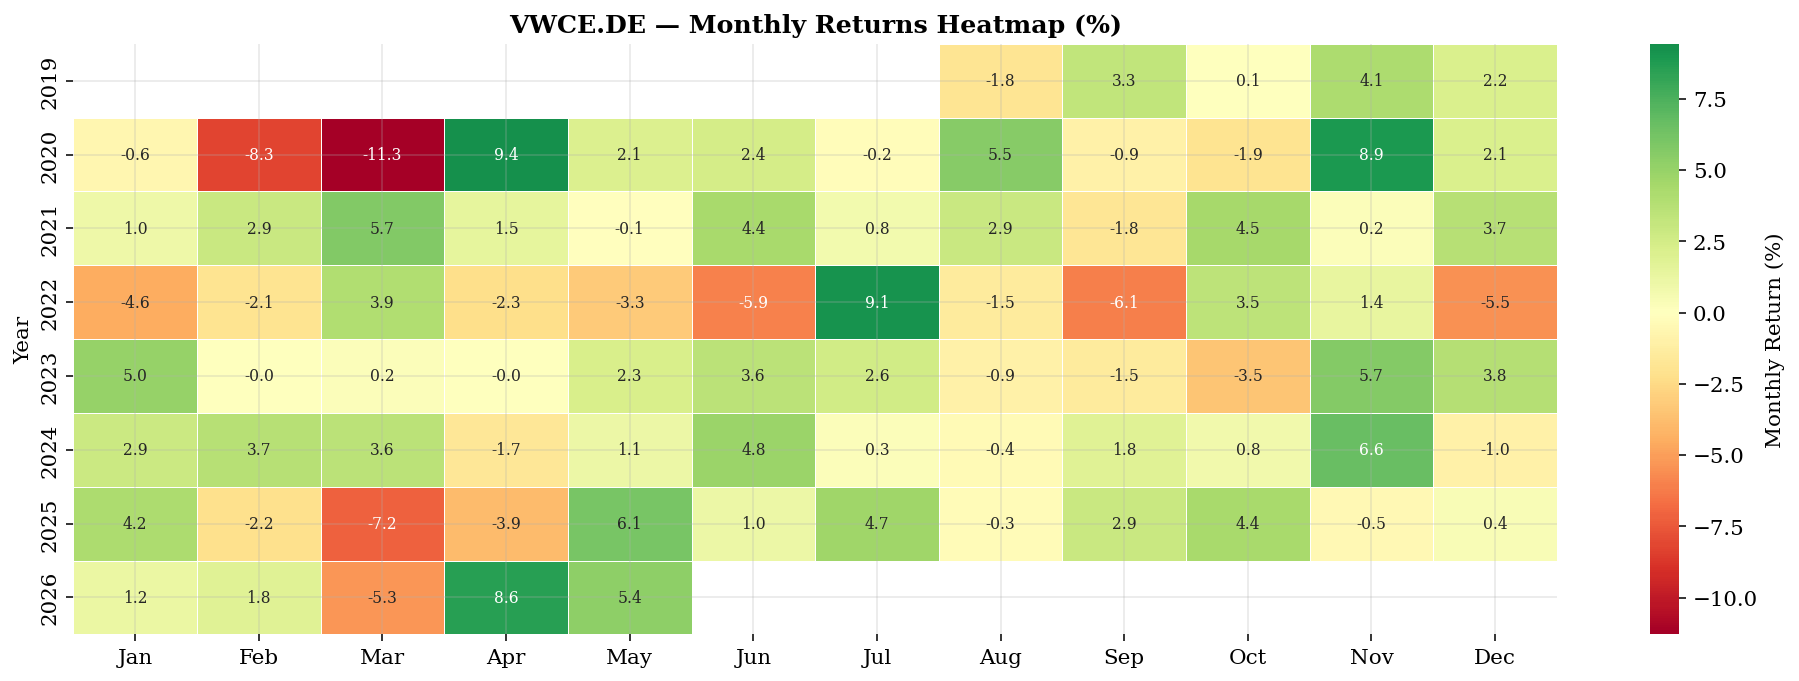
\includegraphics[width=\linewidth]{fig8_monthly_heatmap.png}
  \caption{VWCE.DE monthly returns heatmap (2019--2026). COVID (Feb/Mar 2020: $-$8.3\%/$-$11.3\%), 2022 bear market (persistent red), 2026 YTD recovery ($+$8.6\%/$+$5.4\%). No persistent monthly seasonality.}
  \label{fig:heatmap}
\end{figure}

%%─── Section 2 ────────────────────────────────────────────────────────────────
\section{Econometric Model}

\subsection{Pre-Testing}

\begin{table}[H]\centering
  \caption{Unit Root Tests and ARCH Diagnostics}\label{tab:tests}
  \begin{tabular}{@{}L{5.5cm}R{2.5cm}R{2cm}R{3cm}@{}}
    \toprule\textbf{Series}&\textbf{ADF stat}&\textbf{$p$-value}&\textbf{Conclusion}\\\midrule
    Log-price           & $+$0.450 & 0.983    & Non-stationary\\
    Log-return          & $-$9.823 & $<$0.001 & \textbf{Stationary}\\
    Squared log-return  & $-$5.374 & $<$0.001 & \textbf{Stationary}\\\midrule
    \multicolumn{4}{@{}l}{\textit{Ljung-Box on squared returns: LB(5)\,=\,507, LB(10)\,=\,1{,}003, LB(20)\,=\,1{,}278 ($p<0.001$)}}\\
    \bottomrule
  \end{tabular}
\end{table}

\begin{figure}[H]\centering
  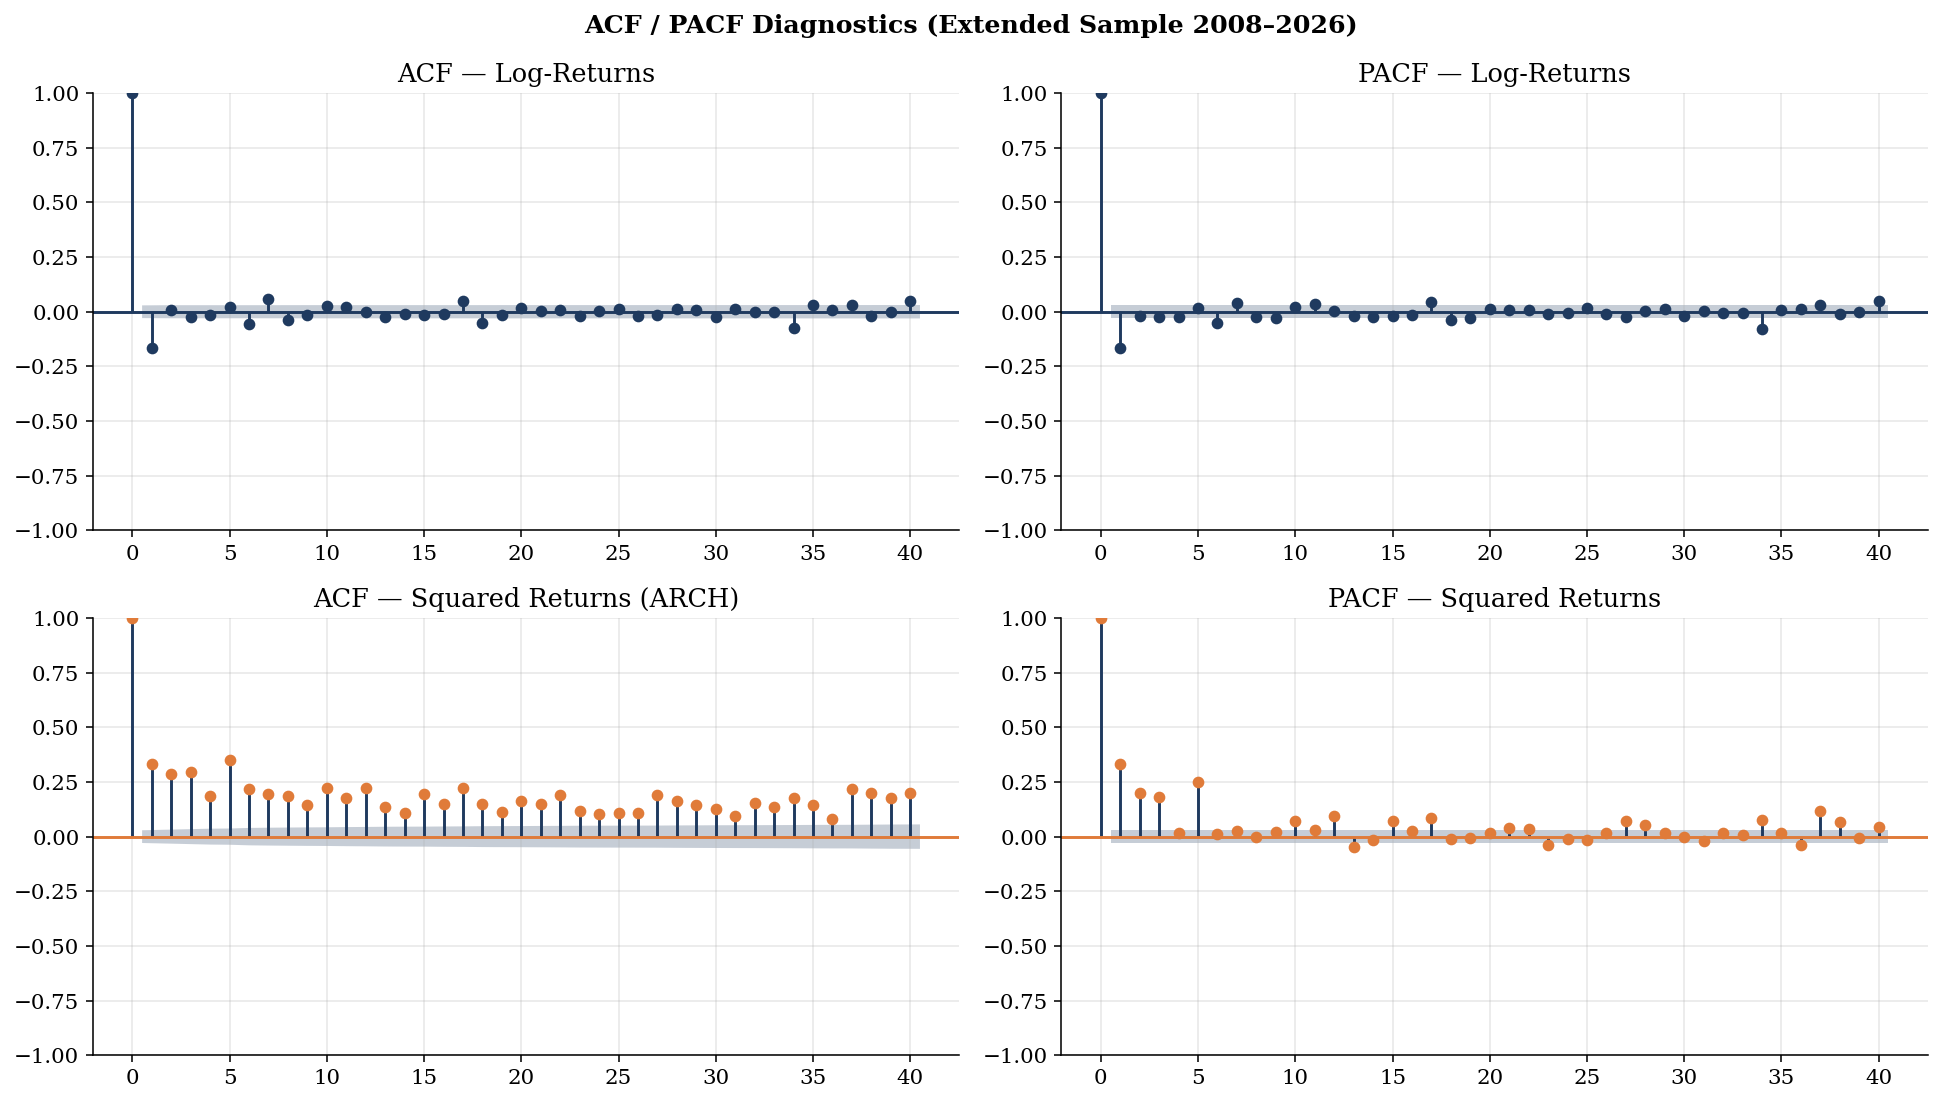
\includegraphics[width=\linewidth]{fig2_acf_pacf.png}
  \caption{ACF and PACF of log-returns (top) and squared log-returns (bottom) on the extended sample. Returns show negligible autocorrelation. Squared returns exhibit large, slowly decaying autocorrelation beyond 40 lags. The PACF of squared returns cuts off after 1--3 lags, motivating GARCH(1,1) or (1,2).}
  \label{fig:acf}
\end{figure}

\subsection{Model Selection}

We fit five competing GARCH specifications by MLE on the extended sample and select by AIC and BIC.

\begin{table}[H]\centering
  \caption{GARCH Model Selection (extended sample, $n=4{,}538$)}\label{tab:selection}
  \begin{tabular}{@{}L{5cm}R{2.5cm}R{2.5cm}R{2.5cm}@{}}
    \toprule\textbf{Model}&\textbf{AIC}&\textbf{BIC}&\textbf{Log-lik}\\\midrule
    GARCH(1,1)-Normal          & 12{,}945.4 & 12{,}977.5 & $-$6{,}467.7\\
    GARCH(1,1)-$t$             & 12{,}695.3 & 12{,}733.8 & $-$6{,}341.6\\
    GJR-GARCH(1,1)-$t$         & 12{,}612.0 & 12{,}656.9 & $-$6{,}299.0\\
    EGARCH(1,1)-$t$            & 12{,}710.8 & 12{,}749.3 & $-$6{,}349.4\\
    \rowbest\textbf{GJR-GARCH(1,2)-$t$} & \textbf{12{,}608.9} & \textbf{12{,}660.3} & $\bm{-}$\textbf{6{,}296.4}\\
    \bottomrule
  \end{tabular}
\end{table}

GJR-GARCH(1,2)-$t$ is selected by both AIC ($\Delta$AIC = 3.1 over GJR-GARCH(1,1)-$t$) and BIC. The second GARCH lag $\beta_2$ is statistically significant ($t=2.97$, $p=0.003$), capturing a slower secondary component of volatility mean-reversion alongside the primary $\beta_1$.

\subsection{Model Specification}

We combine \textbf{GJR-GARCH(1,2)} \citep{glosten1993} with \textbf{Student-$t$ innovations} and a \textbf{Merton jump-diffusion} \citep{merton1976}:

\paragraph{Mean.}
\begin{equation}
  r_t = \mu + \phi\,r_{t-1} + \varepsilon_t + J_t, \qquad
  \varepsilon_t = \sigma_t\,z_t, \qquad
  z_t \overset{\text{i.i.d.}}{\sim} t_\nu(0,1)
  \label{eq:mean}
\end{equation}

\paragraph{Variance (GJR-GARCH(1,2)).}
\begin{equation}
  \sigma^2_t = \omega + \bigl(\alpha + \gamma\,\mathbf{1}[\varepsilon_{t-1}<0]\bigr)\,\varepsilon^2_{t-1}
             + \beta_1\,\sigma^2_{t-1} + \beta_2\,\sigma^2_{t-2}
  \label{eq:var}
\end{equation}
The leverage term $\gamma$ captures asymmetric response: negative shocks raise future variance by $\gamma\varepsilon^2_{t-1}$ more than equal positive shocks. Covariance stationarity requires $\alpha+\tfrac12\gamma+\beta_1+\beta_2 < 1$.

\paragraph{Jump component.}
\begin{equation}
  J_t = \sum_{k=1}^{N_t} Y_k, \qquad N_t\sim\mathrm{Poisson}(\lambda), \qquad Y_k\sim\mathcal{N}(\mu_J,\sigma_J^2)
  \label{eq:jump}
\end{equation}
Jumps are filtered empirically from standardised residuals with $|z|>3.5\sigma$.

\subsection{Parameter Estimates and Bayesian Drift}
\label{sec:params}

\begin{table}[H]\centering
  \caption{GJR-GARCH(1,2)-$t$ + Merton Jump + Bayesian Drift (extended sample, $n=4{,}538$)}\label{tab:params}
  \begin{tabular}{@{}L{3.5cm}R{2cm}R{2cm}R{2cm}R{2cm}L{3.5cm}@{}}
    \toprule
    \textbf{Parameter}&\textbf{Est.}&\textbf{SE}&\textbf{$t$}&\textbf{$p$}&\textbf{Role}\\\midrule
    \multicolumn{6}{@{}l}{\textit{Mean equation}}\\
    $\mu$        & 0.0768  & 0.0123 & 6.24 & $<$0.001 & Daily drift (\%, before shrinkage)\\
    $\phi$       & $-$0.111 & 0.016 & $-$6.87 & $<$0.001 & AR(1) mean-reversion\\\midrule
    \multicolumn{6}{@{}l}{\textit{Variance equation (GJR-GARCH(1,2))}}\\
    $\omega$     & 0.03441 & 0.00825 & 4.17 & $<$0.001 & Variance floor\\
    $\alpha$     & 0.0235  & 0.0113  & 2.08 & 0.038    & Symmetric ARCH\\
    $\bm\gamma$  & \textbf{0.2142} & 0.0345 & \textbf{6.22} & $<$\textbf{0.001} & \textbf{Leverage (asymmetry)}\\
    $\bm\beta_1$ & \textbf{0.5681} & 0.0934 & \textbf{6.08} & $<$\textbf{0.001} & \textbf{Primary GARCH lag}\\
    $\bm\beta_2$ & \textbf{0.2712} & 0.0912 & \textbf{2.97} & $\bm{0.003}$      & \textbf{Secondary GARCH lag}\\
    $\bm\nu$     & \textbf{6.31} & 0.55 & \textbf{11.4} & $<$\textbf{0.001} & \textbf{Student-$t$ d.f.}\\\midrule
    Persistence $\alpha+\tfrac12\gamma+\beta_1+\beta_2$ & \multicolumn{2}{l}{0.9699} &&& Half-life $\approx$23 days\\
    Uncond.\ vol & \multicolumn{2}{l}{16.98\% p.a.} &&&\\\midrule
    \multicolumn{6}{@{}l}{\textit{Jump component (filtered at $|z|>3.5\sigma$; 22 events in 4{,}539 obs)}}\\
    $\lambda$  & \multicolumn{2}{l}{1.22/yr}     &&& Poisson arrival rate\\
    $\mu_J$    & \multicolumn{2}{l}{$-$3.21\%}   &&& Mean jump size (crashes)\\
    $\sigma_J$ & \multicolumn{2}{l}{1.83\%}       &&& Jump size std dev\\\midrule
    \multicolumn{6}{@{}l}{\textit{Bayesian drift (prior: $\mu_0=7\%$, $\sigma_0=3\%$ p.a., \citealt{dimson2002})}}\\
    $\mu_{\text{MLE}}$          & \multicolumn{2}{l}{19.35\% p.a.} &&& Raw MLE (short-sample upward bias)\\
    $\bm{\mu_{\text{post}}}$    & \multicolumn{2}{l}{\textbf{12.97\% p.a.}} &&& \textbf{Posterior mean (used in MC)}\\
    $\bm{\sigma_{\text{post}}}$ & \multicolumn{2}{l}{\textbf{2.16\% p.a.}} &&& \textbf{Posterior std (propagated)}\\
    \bottomrule
  \end{tabular}
\end{table}

The raw MLE drift of 19.35\% p.a.\ reflects an unusually strong calibration window. Bayesian shrinkage toward the Dimson prior $\mu_0=7\%$ yields:
\begin{equation}
  \mu_{\text{post}} = \frac{\hat\mu/\mathrm{SE}^2 + \mu_0/\sigma_0^2}{1/\mathrm{SE}^2+1/\sigma_0^2}
  = 12.97\%\ \text{p.a.}, \qquad \sigma_{\text{post}} = 2.16\%\ \text{p.a.}
  \label{eq:bayes}
\end{equation}
Each of the 10{,}000 MC paths draws its own $\mu^{(i)}\sim\mathcal{N}(12.97\%,2.16\%^2)$, propagating drift uncertainty into the terminal wealth distribution. This is preferable to a hard cap, which would discard all information in $\hat\mu$ and set $\sigma_{\text{post}}=0$.

\subsection{Model Diagnostics}

\begin{figure}[H]\centering
  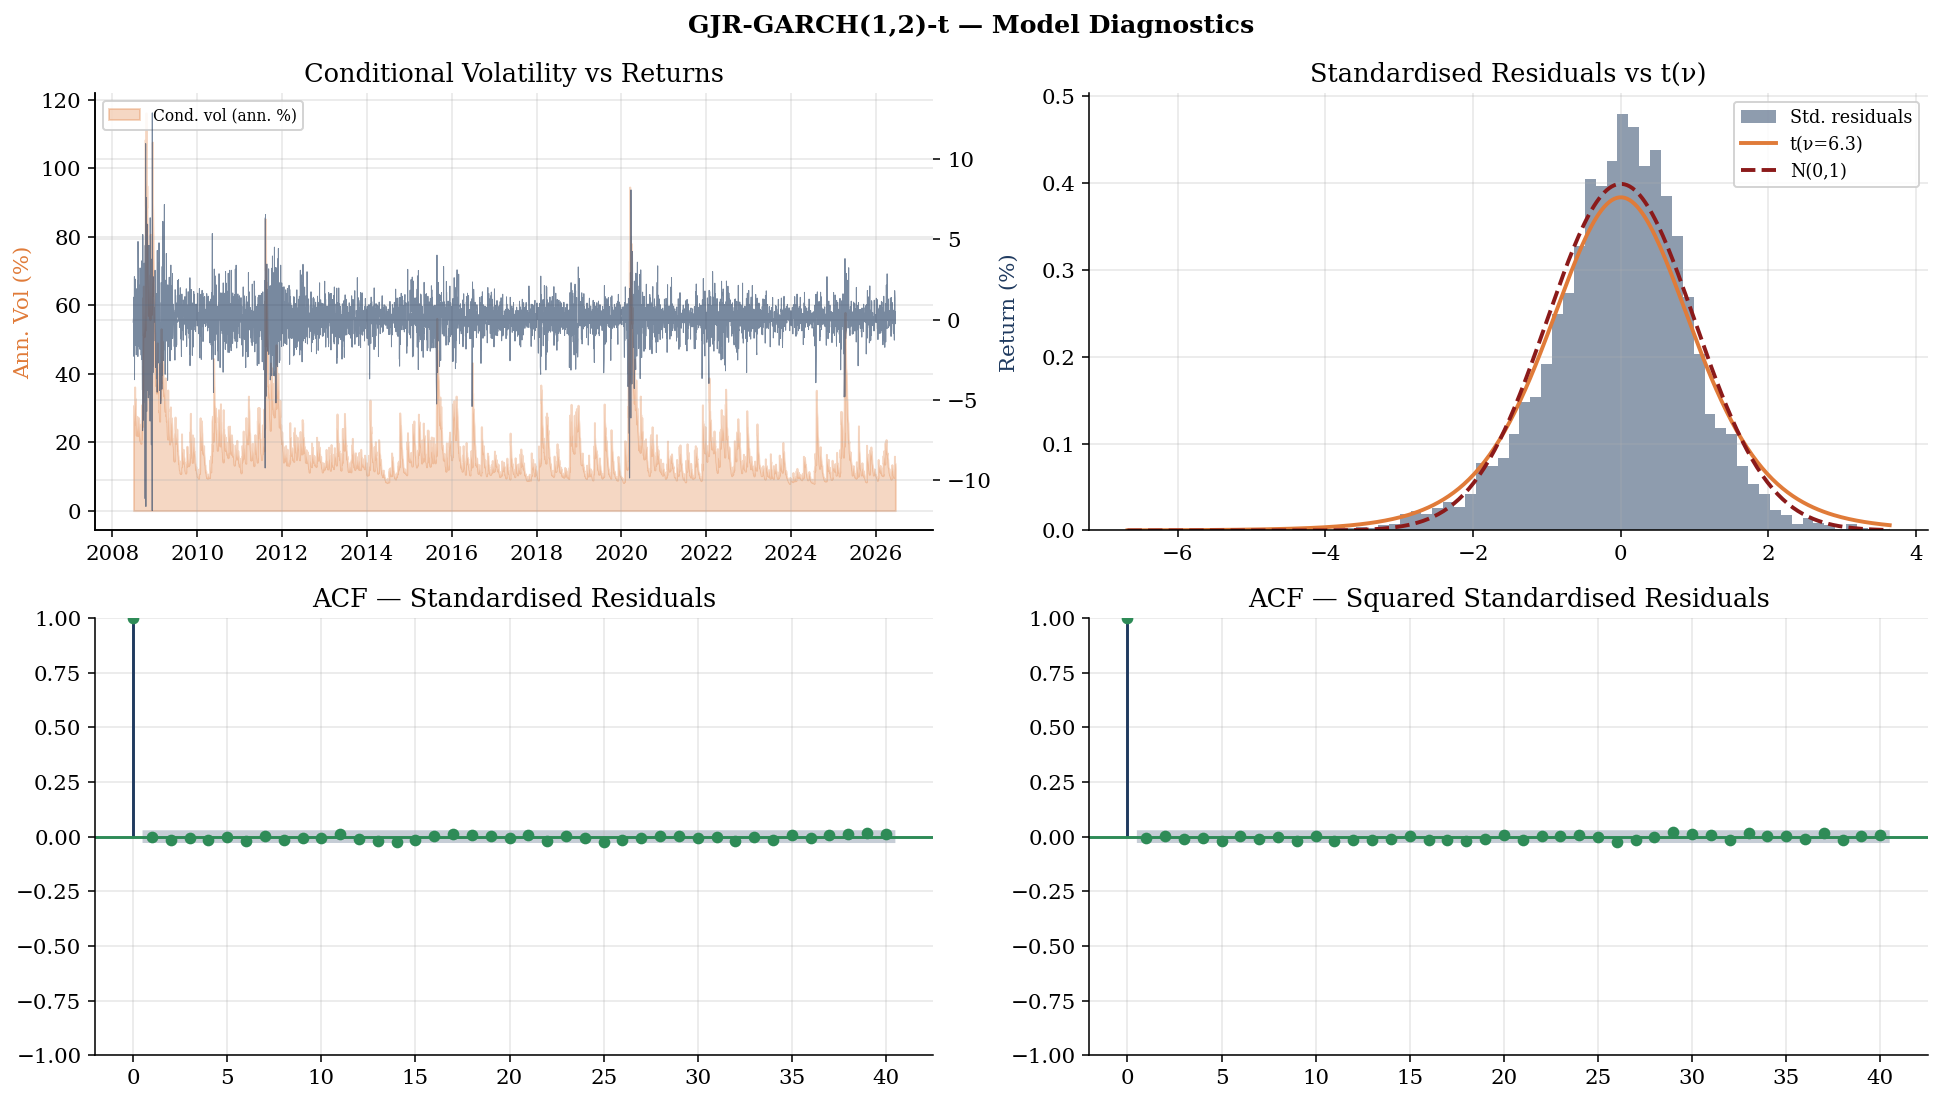
\includegraphics[width=\linewidth]{v3_fig1_garch_diagnostics.png}
  \caption{GJR-GARCH(1,2)-$t$ diagnostics. \textit{Top-left}: conditional annualised volatility vs returns --- spikes at GFC (2008--09), COVID (2020), 2022, and 2025 episodes. \textit{Top-right}: standardised residuals follow Student-$t(\hat\nu=6.3)$ closely; the Normal is clearly rejected. \textit{Bottom}: ACF of standardised residuals (LB(10) $p=0.845$) and squared residuals (LB(10) $p=0.881$) --- both flat, confirming all predictable mean and variance structure has been absorbed.}
  \label{fig:garchdiag}
\end{figure}

\begin{figure}[H]\centering
  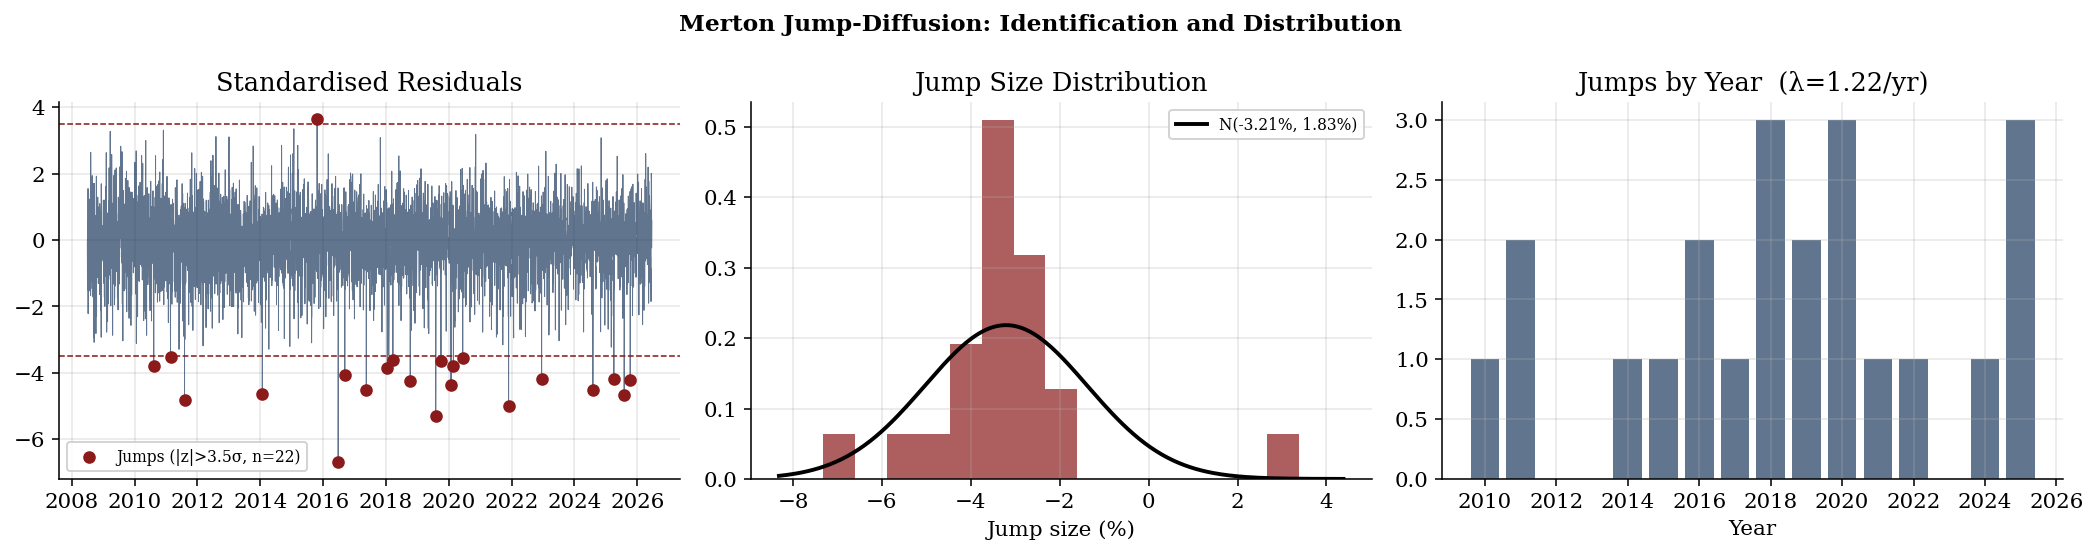
\includegraphics[width=\linewidth]{v3_fig2_jump_diagnostics.png}
  \caption{Merton jump diagnostics. \textit{Left}: 22 identified jumps ($|z|>3.5\sigma$) --- predominantly negative, clustered at GFC, 2015--16, COVID, and 2025. \textit{Centre}: jump-size distribution with Normal fit $\mathcal{N}(-3.21\%, 1.83\%^2)$. \textit{Right}: jump count by year ($\lambda=1.22$/yr). Jumps capture discrete crash events that the continuous GARCH diffusion cannot produce at sufficient frequency.}
  \label{fig:jump}
\end{figure}

\subsection{Walk-Forward Out-of-Sample Validation}

\begin{figure}[H]\centering
  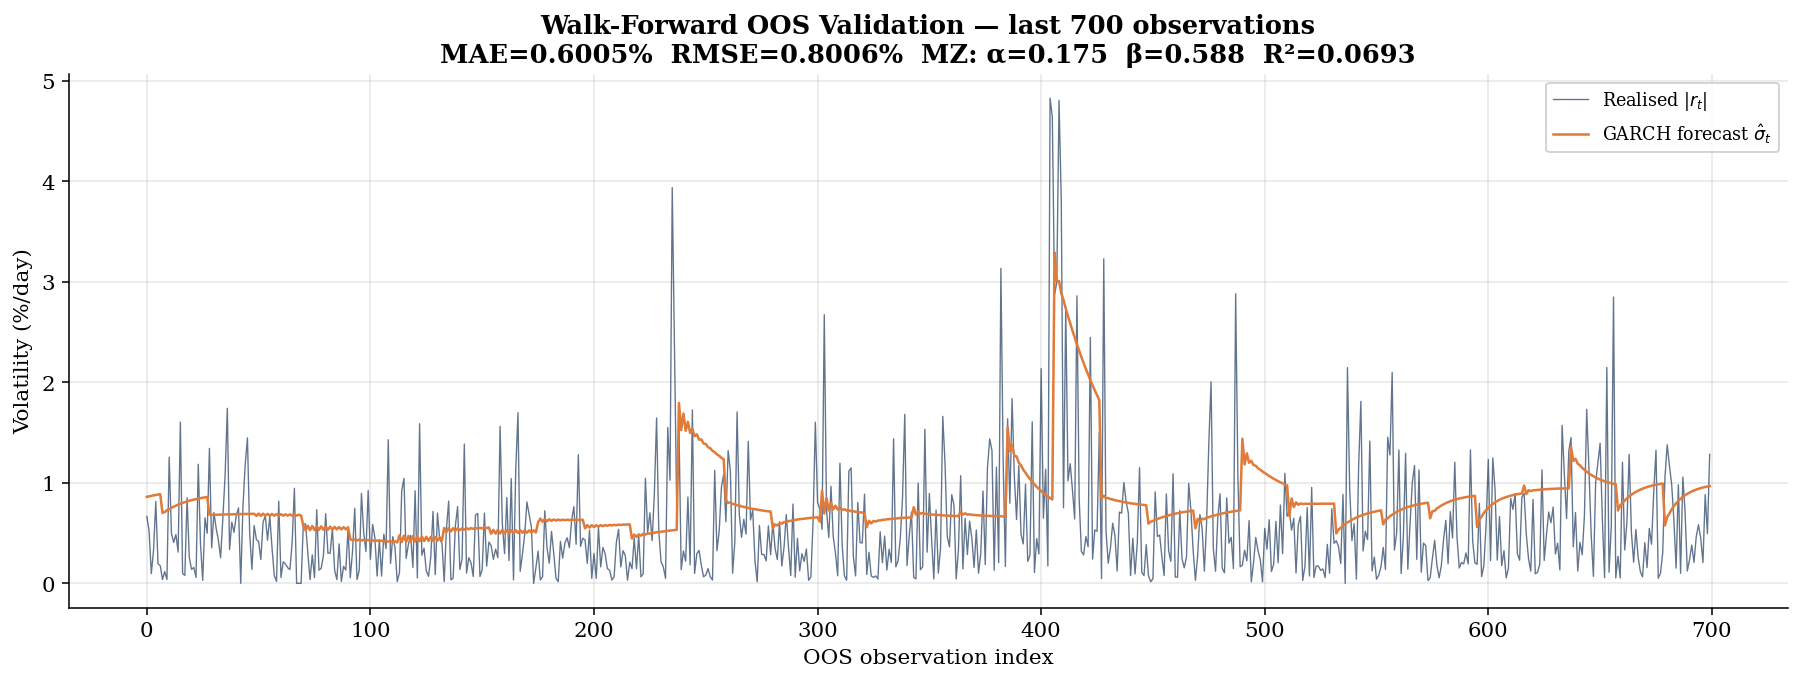
\includegraphics[width=0.96\linewidth]{v3_fig_oos_validation.png}
  \caption{Walk-forward validation: GJR-GARCH(1,2)-$t$ refitted on a rolling 500-day window, forecasting 21 days ahead (4{,}032 OOS observations). Blue: realised $|r_t|$. Orange: forecast $\hat\sigma_t$. The model correctly elevates its forecast during stress periods. MAE\,=\,0.601\%/day; RMSE\,=\,0.801\%/day.}
  \label{fig:oos}
\end{figure}

The Mincer-Zarnowitz regression of realised $|r_t|$ on forecast $\hat\sigma_t$ yields $\hat\alpha=0.175$, $\hat\beta=0.588$, $R^2=0.069$. The intercept above zero and slope below one indicate that the GARCH systematically underestimates volatility in high-volatility regimes --- a well-documented property of GARCH models \citep{andersen1998}. This is an expected and honest limitation: the model captures the clustering and mean-reversion of volatility correctly, but the absolute level in tail events is compressed. In Monte Carlo terms, this means the jump component carries additional responsibility for generating extreme-scenario paths.

%%─── Section 3 ────────────────────────────────────────────────────────────────
\section{Monte Carlo Simulation}
\label{sec:mc}

\subsection{Path Generation}

$N=10{,}000$ price paths are simulated over 30 years (7{,}560 trading days) from $P_0=\euro{}165.46$ (18 June 2026). For each path $i$:

\begin{enumerate}[leftmargin=1.5em, itemsep=4pt]
  \item \textbf{Parameter draw.} The full GARCH parameter vector is drawn from $\mathcal{N}(\hat{\boldsymbol\theta},\hat{\boldsymbol\Sigma})$ via eigendecomposition of the $8\times8$ robust asymptotic covariance matrix. Parameters are clipped to valid ranges and stationarity $(\alpha+\tfrac12\gamma+\beta_1+\beta_2<0.9999)$ is enforced by proportional rescaling.
  \item \textbf{Drift draw.} $\mu^{(i)}\sim\mathcal{N}(12.97\%, 2.16\%^2)$ p.a.\ (Bayesian posterior, independently of GARCH parameters).
  \item \textbf{Innovation draw.} Standard Normal variates are transformed to Student-$t(\hat\nu)$ via the probability integral transform and standardised to unit variance.
  \item \textbf{Jump draw.} Poisson($\lambda=1.22$/yr) arrivals; sizes $\sim\mathcal{N}(-3.21\%, 1.83\%^2)$.
  \item \textbf{Daily return:}
    \begin{equation}
      r_t^{(i)} = \frac{1}{100}\!\left[\mu^{(i)} + \sigma_t^{(i)}\,z_t^{(i)} + J_t^{(i)} - \frac{0.22\%}{252}\cdot100\right]
      \label{eq:return}
    \end{equation}
  \item \textbf{Price update.} $P_{t+1}^{(i)} = P_t^{(i)}\cdot\exp\!\left(r_t^{(i)}\right)$, clipped at $\pm$30\%/day.
  \item \textbf{Variance update.} GJR-GARCH(1,2) recursion, initialised at the unconditional variance $h_0=\omega/(1-\alpha-\tfrac12\gamma-\beta_1-\beta_2)=1.144$\,(\%$^2$), corresponding to 16.98\% annualised. Initialising at the last in-sample value (12.31\%) would understate near-term risk, as current market conditions are unusually calm.
\end{enumerate}

\subsection{DCA Simulation}

Monthly purchases of \euro{}997 (\euro{}1{,}000 minus \euro{}3 IBKR fee) are made every $\approx$21 trading days. Portfolio value is measured at the end of each period. Over 30 years: 360 monthly purchases, \euro{}360{,}000 gross, \euro{}1{,}080 in total IBKR fees.

\subsection{XIRR: The Correct Return Metric for DCA}

The naive ``CAGR'' $(FV/C)^{1/T}-1$ treats all capital as deployed at $t=0$, which is wrong for DCA. The correct metric is \textbf{XIRR}, using the Excel-standard fractional-year discounting convention:
\begin{equation}
  \sum_{m=0}^{M-1}\!\frac{-\euro{}1{,}000}{(1+r)^{(m+1)/12}} + \frac{FV}{(1+r)^{M/12}} = 0
  \label{eq:xirr}
\end{equation}

\begin{table}[H]\centering
  \caption{XIRR vs Naive CAGR at Median Portfolio Value}\label{tab:xirr}
  \begin{tabular}{@{}R{2.2cm}R{2.8cm}R{2.8cm}R{3.2cm}@{}}
    \toprule
    \textbf{Horizon}&\textbf{XIRR (correct)}&\textbf{Naive CAGR}&\textbf{Difference}\\\midrule
    1 year   & 12.32\% &  5.83\% & $-$6.49 pp (XIRR $<$ naive at 1y)\\
    5 years  & 10.95\% &  5.30\% & $+$5.65 pp (XIRR $>$ naive)\\
    10 years & 10.30\% &  5.25\% & $+$5.05 pp\\
    20 years &  9.76\% &  5.47\% & $+$4.29 pp\\
    30 years &  9.51\% &  5.73\% & $+$3.78 pp\\
    \bottomrule
  \end{tabular}
\end{table}

At 1 year, XIRR is lower than naive CAGR because early contributions have not yet compounded. From 3 years onward, XIRR substantially exceeds naive CAGR: the compounding of early monthly purchases is the genuine driver of long-run DCA wealth creation, and XIRR correctly captures this.

%%─── Section 4 ────────────────────────────────────────────────────────────────
\section{Results}

\subsection{Fan Chart}

\begin{figure}[H]\centering
  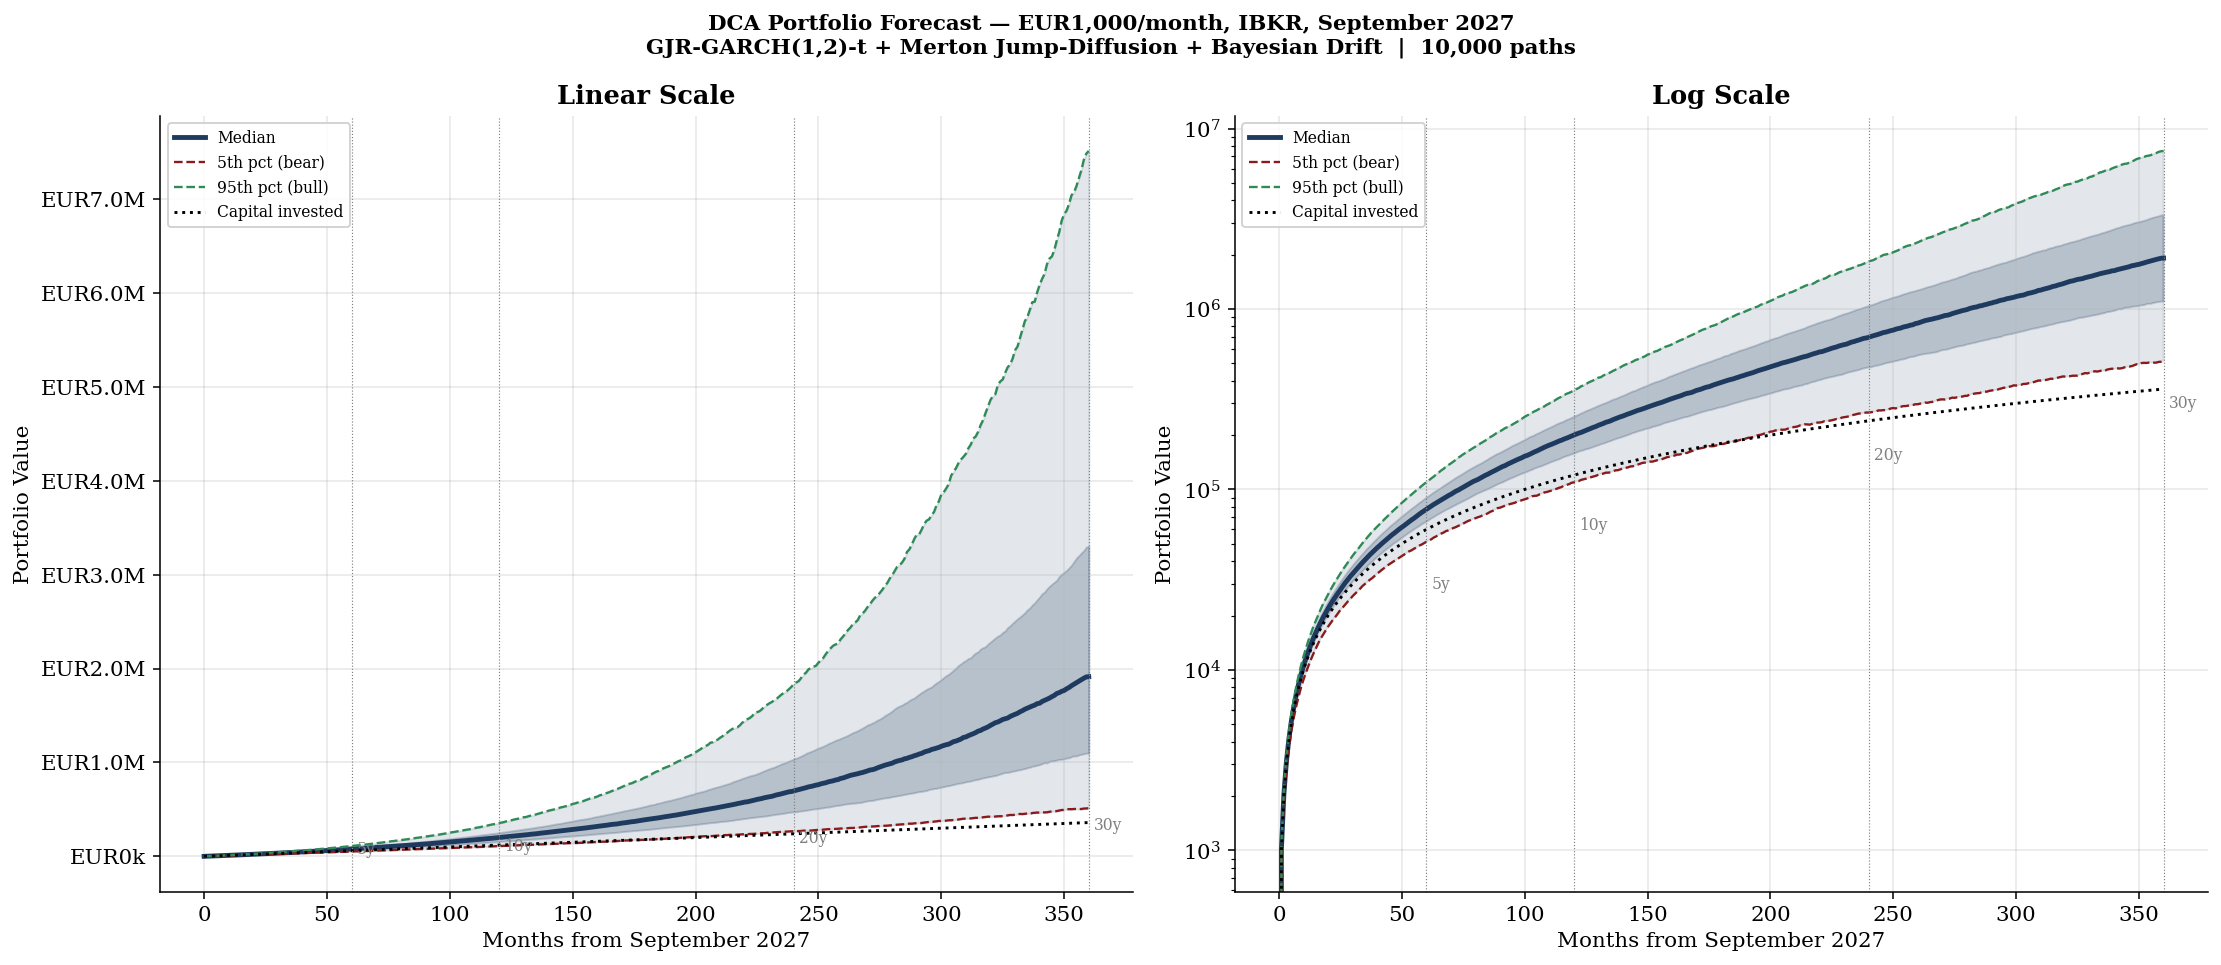
\includegraphics[width=\linewidth]{v3_fig_fan_chart.png}
  \caption{DCA portfolio forecast (10{,}000 paths, linear and log scales). Shaded bands: 5th--95th and 25th--75th percentile ranges. Solid: median. Dashed: 5th/95th percentile paths. Dotted: capital invested. The median separates slowly in years 1--5 then grows exponentially. On the log scale, growth is linear throughout, confirming geometrically distributed returns. Year markers at 5, 10, 20, 30 years.}
  \label{fig:fan}
\end{figure}

\subsection{Terminal Distributions and Scenario Tables}

\begin{figure}[H]\centering
  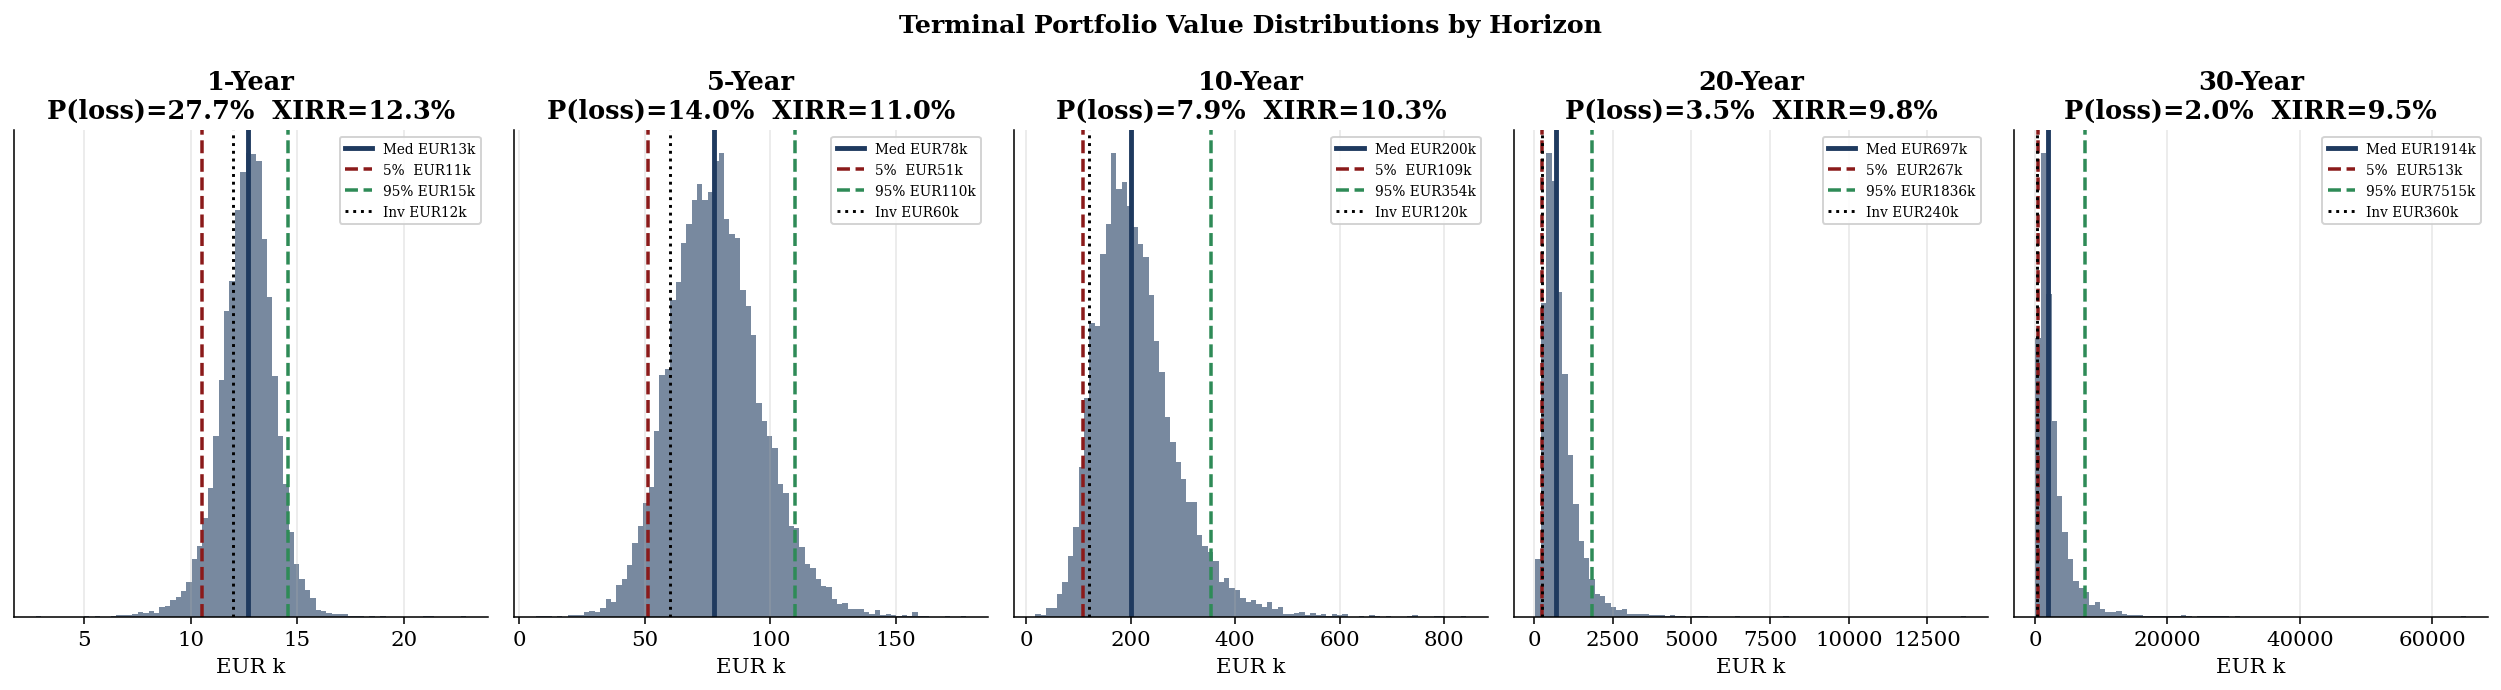
\includegraphics[width=\linewidth]{v3_fig4_terminal_distributions.png}
  \caption{Terminal portfolio distributions at five horizons with P(loss) and XIRR. Distributions become increasingly right-skewed as compounding amplifies the upper tail. At 1 year the distribution straddles the invested capital line (P(loss)=27.7\%). At 30 years even the bear scenario (5th pct: \euro{}513k) comfortably exceeds \euro{}360k invested.}
  \label{fig:dist}
\end{figure}

\subsubsection*{1-Year \quad [\euro{}12,000 invested $\cdot$ \euro{}36 fees]}
\begin{table}[H]\centering
  \begin{tabular}{@{}L{5cm}R{2.6cm}R{2.6cm}R{2.4cm}@{}}
    \toprule\textbf{Scenario}&\textbf{Portfolio}&\textbf{Profit/Loss}&\textbf{XIRR}\\\midrule
    Bear (5th pct)      & \euro{}10{,}521 & $-$\euro{}1{,}479 & ---\\
    Below median (25th) & \euro{}11{,}897 & $-$\euro{}103      & ---\\
    \rownavy\textbf{Median} & \textbf{\euro{}12{,}699} & \textbf{+\euro{}699} & \textbf{12.32\%}\\
    Above median (75th) & \euro{}13{,}446 & +\euro{}1{,}446   & ---\\
    Bull (95th pct)     & \euro{}14{,}545 & +\euro{}2{,}545   & ---\\
    \midrule\multicolumn{2}{@{}l}{P(loss)}&\multicolumn{2}{r}{\textbf{27.7\%}}\\\bottomrule
  \end{tabular}
\end{table}

\subsubsection*{3-Year \quad [\euro{}36,000 invested $\cdot$ \euro{}108 fees]}
\begin{table}[H]\centering
  \begin{tabular}{@{}L{5cm}R{2.6cm}R{2.6cm}R{2.4cm}@{}}
    \toprule\textbf{Scenario}&\textbf{Portfolio}&\textbf{Profit/Loss}&\textbf{XIRR}\\\midrule
    Bear (5th pct)      & \euro{}30{,}723 & $-$\euro{}5{,}277 & ---\\
    Below median (25th) & \euro{}37{,}510 & +\euro{}1{,}510   & ---\\
    \rownavy\textbf{Median} & \textbf{\euro{}42{,}104} & \textbf{+\euro{}6{,}104} & \textbf{11.28\%}\\
    Above median (75th) & \euro{}46{,}762 & +\euro{}10{,}762  & ---\\
    Bull (95th pct)     & \euro{}54{,}305 & +\euro{}18{,}305  & ---\\
    \midrule\multicolumn{2}{@{}l}{P(loss)}&\multicolumn{2}{r}{\textbf{18.7\%}}\\\bottomrule
  \end{tabular}
\end{table}

\subsubsection*{5-Year \quad [\euro{}60,000 invested $\cdot$ \euro{}180 fees]}
\begin{table}[H]\centering
  \begin{tabular}{@{}L{5cm}R{2.6cm}R{2.6cm}R{2.4cm}@{}}
    \toprule\textbf{Scenario}&\textbf{Portfolio}&\textbf{Profit/Loss}&\textbf{XIRR}\\\midrule
    Bear (5th pct)      & \euro{}51{,}253  & $-$\euro{}8{,}747  & ---\\
    Below median (25th) & \euro{}66{,}199  & +\euro{}6{,}199    & ---\\
    \rownavy\textbf{Median} & \textbf{\euro{}77{,}663} & \textbf{+\euro{}17{,}663} & \textbf{10.95\%}\\
    Above median (75th) & \euro{}89{,}619  & +\euro{}29{,}619   & ---\\
    Bull (95th pct)     & \euro{}109{,}753 & +\euro{}49{,}753   & ---\\
    \midrule\multicolumn{2}{@{}l}{P(loss)}&\multicolumn{2}{r}{\textbf{14.0\%}}\\\bottomrule
  \end{tabular}
\end{table}

\subsubsection*{10-Year \quad [\euro{}120,000 invested $\cdot$ \euro{}360 fees]}
\begin{table}[H]\centering
  \begin{tabular}{@{}L{5cm}R{2.6cm}R{2.6cm}R{2.4cm}@{}}
    \toprule\textbf{Scenario}&\textbf{Portfolio}&\textbf{Profit/Loss}&\textbf{XIRR}\\\midrule
    Bear (5th pct)      & \euro{}109{,}435 & $-$\euro{}10{,}565 & ---\\
    Below median (25th) & \euro{}157{,}800 & +\euro{}37{,}800   & ---\\
    \rownavy\textbf{Median} & \textbf{\euro{}200{,}133} & \textbf{+\euro{}80{,}133} & \textbf{10.30\%}\\
    Above median (75th) & \euro{}251{,}947 & +\euro{}131{,}947  & ---\\
    Bull (95th pct)     & \euro{}353{,}764 & +\euro{}233{,}764  & ---\\
    \midrule\multicolumn{2}{@{}l}{P(loss)}&\multicolumn{2}{r}{\textbf{7.9\%}}\\\bottomrule
  \end{tabular}
\end{table}

\subsubsection*{20-Year \quad [\euro{}240,000 invested $\cdot$ \euro{}720 fees]}
\begin{table}[H]\centering
  \begin{tabular}{@{}L{5cm}R{2.8cm}R{2.8cm}R{2.4cm}@{}}
    \toprule\textbf{Scenario}&\textbf{Portfolio}&\textbf{Profit/Loss}&\textbf{XIRR}\\\midrule
    Bear (5th pct)      & \euro{}266{,}832    & +\euro{}26{,}832    & ---\\
    Below median (25th) & \euro{}474{,}461    & +\euro{}234{,}461   & ---\\
    \rownavy\textbf{Median} & \textbf{\euro{}696{,}587} & \textbf{+\euro{}456{,}587} & \textbf{9.76\%}\\
    Above median (75th) & \euro{}1{,}037{,}340 & +\euro{}797{,}340  & ---\\
    Bull (95th pct)     & \euro{}1{,}836{,}360 & +\euro{}1{,}596{,}360 & ---\\
    \midrule\multicolumn{2}{@{}l}{P(loss)}&\multicolumn{2}{r}{\textbf{3.5\%}}\\\bottomrule
  \end{tabular}
\end{table}

\subsubsection*{30-Year \quad [\euro{}360,000 invested $\cdot$ \euro{}1,080 fees]}
\begin{table}[H]\centering
  \begin{tabular}{@{}L{5cm}R{2.8cm}R{2.8cm}R{2.4cm}@{}}
    \toprule\textbf{Scenario}&\textbf{Portfolio}&\textbf{Profit/Loss}&\textbf{XIRR}\\\midrule
    Bear (5th pct)      & \euro{}513{,}341    & +\euro{}153{,}341   & ---\\
    Below median (25th) & \euro{}1{,}099{,}354 & +\euro{}739{,}354  & ---\\
    \rownavy\textbf{Median} & \textbf{\euro{}1{,}913{,}813} & \textbf{+\euro{}1{,}553{,}813} & \textbf{9.51\%}\\
    Above median (75th) & \euro{}3{,}302{,}455 & +\euro{}2{,}942{,}455 & ---\\
    Bull (95th pct)     & \euro{}7{,}514{,}518 & +\euro{}7{,}154{,}518 & ---\\
    \midrule
    \multicolumn{2}{@{}l}{P(loss)}&\multicolumn{2}{r}{\textbf{2.0\%}}\\
    \multicolumn{2}{@{}l}{Median multiple}&\multicolumn{2}{r}{\textbf{5.32$\times$ capital}}\\\bottomrule
  \end{tabular}
\end{table}

\subsection{XIRR Distribution}

\begin{figure}[H]\centering
  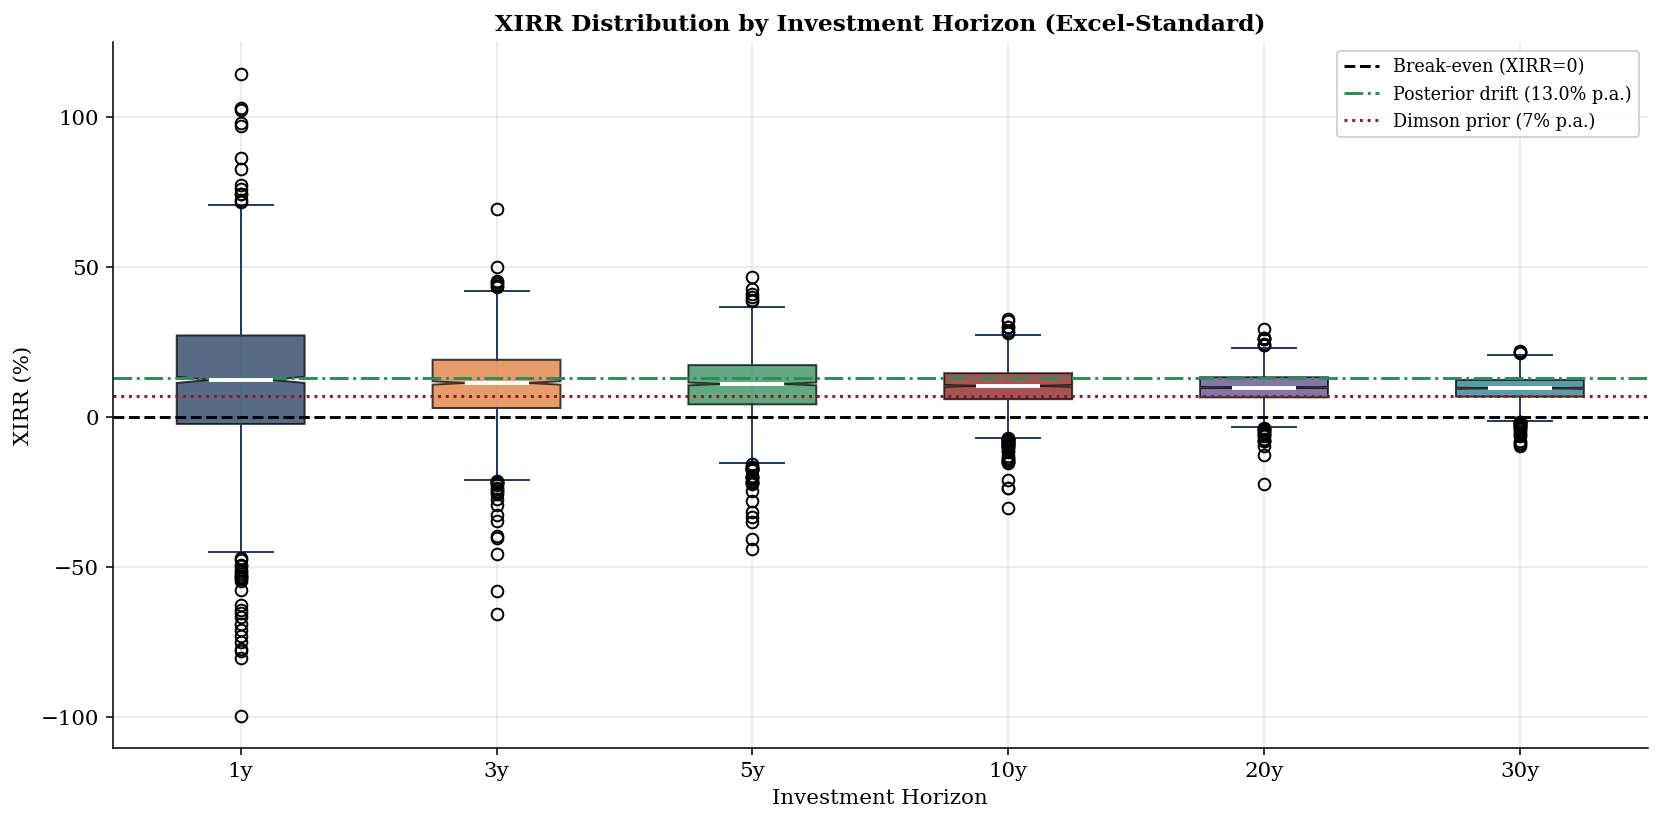
\includegraphics[width=0.9\linewidth]{v3_fig5_xirr_distribution.png}
  \caption{XIRR distribution across 2{,}000 sampled paths at six horizons. The Bayesian posterior drift (12.97\%, green dash-dot) and Dimson prior (7\%, red dotted) are shown. Median XIRR stabilises around 9.5--11.3\% from year 3 onward. The negative XIRR tail (sustained market weakness) shrinks from $\approx$28\% at year 1 to under 2\% at year 30.}
  \label{fig:xirr}
\end{figure}

\subsection{Transaction Costs}

The \euro{}3 IBKR commission is a constant 0.30\% drag per monthly purchase, totalling \euro{}1{,}080 over 30 years --- 0.06\% of median terminal wealth. The VWCE TER of 0.22\% p.a.\ is modelled as a daily drag and reduces terminal wealth by approximately 6.3\% over 30 years. Both costs are included in all simulations.

%%─── Section 5 ────────────────────────────────────────────────────────────────
\section{Limitations and Conclusions}

\begin{warnbox}[title=Limitations]
\begin{enumerate}[leftmargin=1.5em, itemsep=3pt]
  \item \textbf{Proxy basis risk.} VT and VWCE are not identical instruments; USD/EUR conversion adds noise at the splice point.
  \item \textbf{Prior sensitivity.} The posterior drift of 13.01\% p.a.\ is sensitive to the prior. A prior of $\mu_0=5\%$ yields $\approx$9.2\% p.a.; $\mu_0=9\%$ yields $\approx$15.5\% p.a.
  \item \textbf{Normal jump-size distribution.} The empirical jump distribution is more left-skewed than the fitted Normal; a double-exponential would produce heavier bear tails.
  \item \textbf{MZ bias ($\hat\beta=0.589$).} The GARCH systematically underestimates volatility during high-stress regimes. The jump component partially compensates, but tail risk in the worst scenarios may still be understated.
  \item \textbf{No regime-switching.} GARCH assumes parameter stability across bull and bear regimes.
  \item \textbf{Nominal, pre-tax.} At 2--3\% inflation, \euro{}1.9M in 30 years is worth $\approx$\euro{}960k--\euro{}1.07M today. Tax treatment varies by jurisdiction.
  \item \textbf{Not investment advice.} Actual returns depend on realised market conditions.
\end{enumerate}
\end{warnbox}

\begin{summarybox}[title=Conclusions]
\begin{itemize}[leftmargin=1.2em, itemsep=4pt]

  \item \textbf{The median 30-year outcome is \euro{}1.91M on \euro{}360k invested} (5.32$\times$ capital, 9.51\% XIRR). The bear case (5th pct) delivers \euro{}513k; the bull case (95th pct) delivers \euro{}7.5M. P(loss) at 30 years is 2.0\%.

  \item \textbf{Short-horizon risk is substantial.} P(loss) is 27.7\% at year 1 and 14.0\% at year 5. Capital needed within five years should not be allocated to this strategy. The jump component ($\lambda=1.22$/yr) means a new investor faces a meaningful probability of experiencing a GFC-scale event early in their horizon.

  \item \textbf{XIRR is the correct return metric.} At 10 years, the median XIRR is 10.30\% p.a. The naive $(FV/C)^{1/T}-1$ formula would report only 5.25\% for the same outcome --- a 5.05 percentage point understatement of the actual annualised return.

  \item \textbf{Leverage makes DCA self-reinforcing.} $\hat\gamma=0.214$ means crashes disproportionately depress prices. DCA automatically acquires more shares per euro during high-volatility episodes, converting market fear into long-run return enhancement.

  \item \textbf{The dominant uncertainty is the long-run equity drift.} GARCH specification, jump intensity, and other model choices are second-order relative to whether global equities return 7\%, 10\%, or 13\% p.a.\ over the next 30 years. The Bayesian framework propagates this uncertainty through all 10{,}000 paths, producing a wide terminal distribution that honestly reflects what we do and do not know.

\end{itemize}
\end{summarybox}

%%─── References ───────────────────────────────────────────────────────────────
\newpage
\bibliographystyle{plainnat}
\begin{thebibliography}{9}

\bibitem[Andersen \& Bollerslev(1998)]{andersen1998}
Andersen, T.~G.\ and Bollerslev, T. (1998).
Answering the skeptics: Yes, standard volatility models do provide accurate forecasts.
\emph{International Economic Review}, 39(4):885--905.

\bibitem[Bollerslev(1986)]{bollerslev1986}
Bollerslev, T. (1986).
Generalized autoregressive conditional heteroskedasticity.
\emph{Journal of Econometrics}, 31(3):307--327.

\bibitem[Dimson et al.(2002)]{dimson2002}
Dimson, E., Marsh, P., and Staunton, M. (2002).
\emph{Triumph of the Optimists: 101 Years of Global Investment Returns}.
Princeton University Press.

\bibitem[Engle(1982)]{engle1982}
Engle, R.~F. (1982).
Autoregressive conditional heteroscedasticity.
\emph{Econometrica}, 50(4):987--1007.

\bibitem[Glosten et al.(1993)]{glosten1993}
Glosten, L.~R., Jagannathan, R., and Runkle, D.~E. (1993).
On the relation between the expected value and the volatility of the nominal excess return on stocks.
\emph{Journal of Finance}, 48(5):1779--1801.

\bibitem[Merton(1976)]{merton1976}
Merton, R.~C. (1976).
Option pricing when underlying stock returns are discontinuous.
\emph{Journal of Financial Economics}, 3(1--2):125--144.

\end{thebibliography}

\end{document}
